
% xetex expected
\documentclass[xetex,professionalfont]{beamer}

% we want math
\usepackage{amsmath}

% fixes and extensions to amsmath
\usepackage{mathtools}

% additional math symbols
\usepackage{amssymb}

% good-looking fractions in text via \sfrac
\usepackage{xfrac}

% fix spaces after custom commands (see below for examples)
\usepackage{xspace}

% minted allows for fancy syntax highlighting (requires python with pygments)
% usage:
%   \begin{minted}{python}
%   codeb
%   \end{minted}
\usepackage{minted}

% better looking tables
% usage:
%   begin with a \toprule, write a single row of column headings,
%   then add \midrule and after the columns of data we finish with \bottomrule
% example:
%   \begin{tabular}{llr} \toprule
%   Animal & Description & Price \midrule
%   cat & foo & 10 \\
%   dog & bar & 20 \\ \bottomrule
%   \end{tabular}
% note that good tables generally neither have vertical rules nor double rules
\usepackage{booktabs}

% system font support (requires xetex or luatex)
\usepackage{fontspec}
\setmonofont[Scale=0.7]{Cousine} % part of ttf-chromeos fonts on Arch

% improve microtypography
\usepackage{microtype}

% multi-language quotes for babel
\usepackage{csquotes}

% easy way to include copyright information
\usepackage{copyrightbox}

% better bibliographies
\usepackage[backend=biber,style=authoryear]{biblatex}

% language support (english,ngerman)
\usepackage[english]{babel}

% process diagrams (part of texlive-pictures)
\usepackage{smartdiagram}

% plots
\usepackage{pgfplots}

% -----------------------------------------------------------------------------

% specify PDF metadata
\hypersetup{pdftitle={CVSP VO - Category Recognition 2 - Deep Learning},pdfsubject={},pdfauthor={Christopher Pramerdorfer}}

% copyright font style
\makeatletter\renewcommand{\CRB@setcopyrightfont}{\tiny\color{lightgray}}

% make emph bold
\DeclareTextFontCommand{\emph}{\bfseries}

% use proper fonts for math
% \usefonttheme[onlymath]{serif}

% use tuwcvl beamer theme
\usetheme{tuwcvl}

% add bib file
\addbibresource{literature.bib}

% diagram style

\smartdiagramset{norm/.style={
	 sequence item border color=gray!30!black,
	 sequence item border size=1.5\pgflinewidth,
	 sequence item font size=\footnotesize,
  }
}

\smartdiagramset{transp/.style={
	 sequence item border color=gray!70!black,
	 sequence item border size=1.5\pgflinewidth,
	 sequence item font size=\footnotesize,
	 sequence item fill opacity=0.5,
	 sequence item text opacity=0.5
  }
}

\smartdiagramset{norm}

% plot setup

\pgfplotsset{width=8cm}

% -----------------------------------------------------------------------------

% common english abbreviations
\newcommand{\ie}{\mbox{i.e.}\xspace} % i.e.
\newcommand{\eg}{\mbox{e.g.}\xspace} % e.g.

% math - argmin and argmax
\DeclareMathOperator*{\argmin}{arg\,min}
\DeclareMathOperator*{\argmax}{arg\,max}

% shortcuts for number ranges
\newcommand{\NN}{\mathbb{N}}
\newcommand{\ZZ}{\mathbb{Z}}
\newcommand{\QQ}{\mathbb{Q}}
\newcommand{\RR}{\mathbb{R}}

% bold vectors
\renewcommand{\vec}[1]{\ensuremath{\mathbf{#1}}}

% vector shortcuts
\newcommand{\va}{\vec{a}}
\newcommand{\vb}{\vec{b}}
\newcommand{\vc}{\vec{c}}
\newcommand{\ve}{\vec{e}}
\newcommand{\vr}{\vec{r}}
\newcommand{\vs}{\vec{s}}
\newcommand{\vt}{\vec{t}}
\newcommand{\vu}{\vec{u}}
\newcommand{\vv}{\vec{v}}
\newcommand{\vw}{\vec{w}}
\newcommand{\vx}{\vec{x}}
\newcommand{\vy}{\vec{y}}
\newcommand{\vz}{\vec{z}}

% -----------------------------------------------------------------------------

\title{Computer Vision Systems Programming VO}
\subtitle{Deep Learning}
\author{Christopher Pramerdorfer}
\institute{Computer Vision Lab, Vienna University of Technology}

\begin{document}

% disable minted's syntax checks
\expandafter\def\csname PY@tok@err\endcsname{}

% -----------------------------------------------------------------------------

\begin{frame}
\maketitle
\end{frame}

% -----------------------------------------------------------------------------

\begin{frame}
\frametitle{Topics}

Deep learning motivation\\\medskip
Multilayer perceptrons\\\medskip
Pylearn2 library\\\medskip
Convolutional neural networks\\\medskip
Deep learning applications

\bigskip
\begin{center}
	\copyrightbox[b]
	{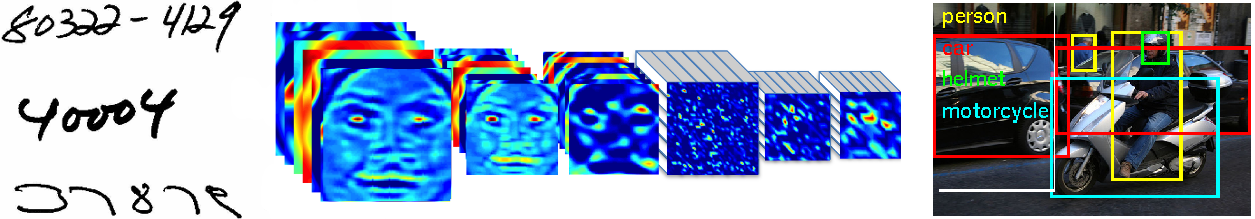
\includegraphics[width=10cm]{figures/intro-collage.png}}
	{\centering Images from \cite{lecun1989}, \cite{taigman2013}, \url{image-net.org}}
\end{center}

\end{frame}

% -----------------------------------------------------------------------------

\begin{frame}
\frametitle{Object Recognition}
\framesubtitle{Traditional Approach}

\begin{center}
\smartdiagram[sequence diagram]{Image,Feature Extraction,Learned Mapping}\\\bigskip % learned mapping maps from the representation to the output, such as a class label
\smartdiagramset{transp}
\smartdiagram[sequence diagram]{Image,SIFT+BOW,SVM}
\end{center}

\end{frame}

% -----------------------------------------------------------------------------

\begin{frame}
\frametitle{Object Recognition}
\framesubtitle{Traditional Approach}

Problem: how to choose the representation/features? % the representation comprises all features

\bigskip
\enquote{General} features not optimal
\begin{itemize}
	\item Not tuned to task at hand, low-level
\end{itemize}

\bigskip
Designing task-specific features is complex
\begin{itemize}
	\item Virtually impossible to do optimally
\end{itemize}

\end{frame}

% -----------------------------------------------------------------------------

\begin{frame}
\frametitle{Object Recognition}
\framesubtitle{Deep Learning}

Solution: learn representation as well\\\medskip % this is called ... representation learning
Learning high-level representations directly is difficult

\bigskip
Deep Learning (DL) solves this
\begin{itemize}
	\item By learning a hierarchy of representations % hence "deep" / hierarchy is fixed, everything else is learned
	\item Layers in hierarchy build upon each other % from low-level to high-level representation
\end{itemize}

\end{frame}

% -----------------------------------------------------------------------------

\begin{frame}
\frametitle{Object Recognition}
\framesubtitle{Deep Learning}

\begin{center}
	\copyrightbox[b]
	{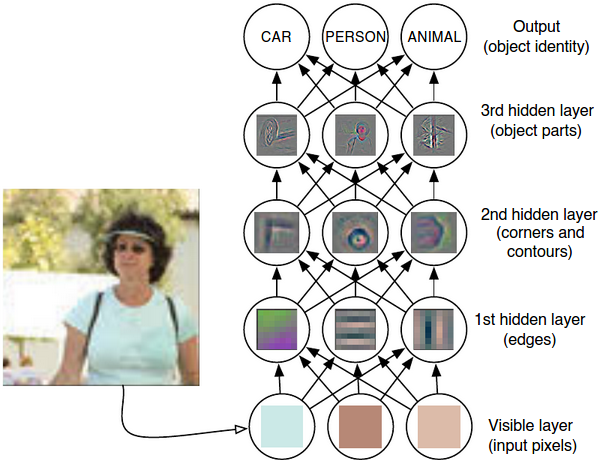
\includegraphics[width=7.5cm]{figures/dl-layer-example.png}}
	{\centering Image from \cite{bengio2014}}
\end{center}

\end{frame}

% -----------------------------------------------------------------------------

\begin{frame}
\frametitle{Object Recognition}
\framesubtitle{Deep Learning}

$n$ levels of features/representations\\\medskip
Learned jointly with the output mapping

\bigskip
\begin{center}
\smartdiagramset{sequence item text width=1cm}
\smartdiagram[sequence diagram]{Image,LF $1$,$\dots$,LF $n$,LM}
\end{center}

\end{frame}

% -----------------------------------------------------------------------------

\begin{frame}
\frametitle{Multilayer Perceptrons}

DL is usually realized using MultiLayer Perceptrons (MLPs) % also known as feed-forward neural networks

\bigskip
\begin{center}
	\copyrightbox[b]
	{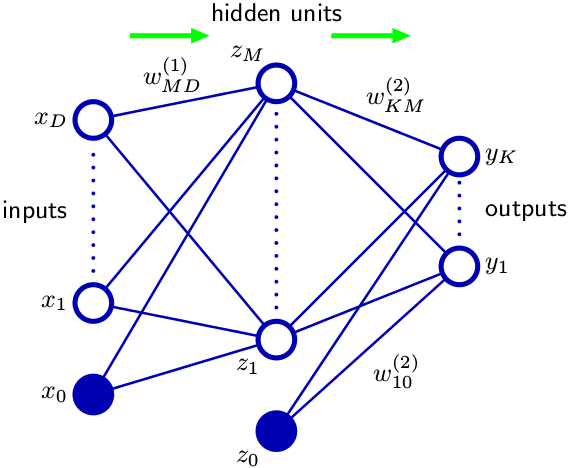
\includegraphics[width=4.5cm]{figures/two-layer-mlp.png}}
	{\centering Image from \cite{bishop2006}}
\end{center}

\end{frame}

% -----------------------------------------------------------------------------

\begin{frame}
\frametitle{Multilayer Perceptrons}
\framesubtitle{The Perceptron}

Binary linear classifier\\\medskip
Feature vectors $\vx$ classified as $f(\vw^\top\vx+b)\in\{-1,+1\}$\\\medskip % sometimes {0,1} is used, but {-1,1} facilitates training
$f$ is a discontinuous step function % so f is not differentiable
\[
f(v)=\begin{cases}
	+1 & \text{if } v>0\\
	-1 & \text{otherwise}
\end{cases}
\]\\\medskip
$\vw,b$ learned from training data % the decision hyperplane is wx+b=0

\end{frame}

% -----------------------------------------------------------------------------

\begin{frame}
\frametitle{Multilayer Perceptrons}
\framesubtitle{The Perceptron}

\begin{center}
	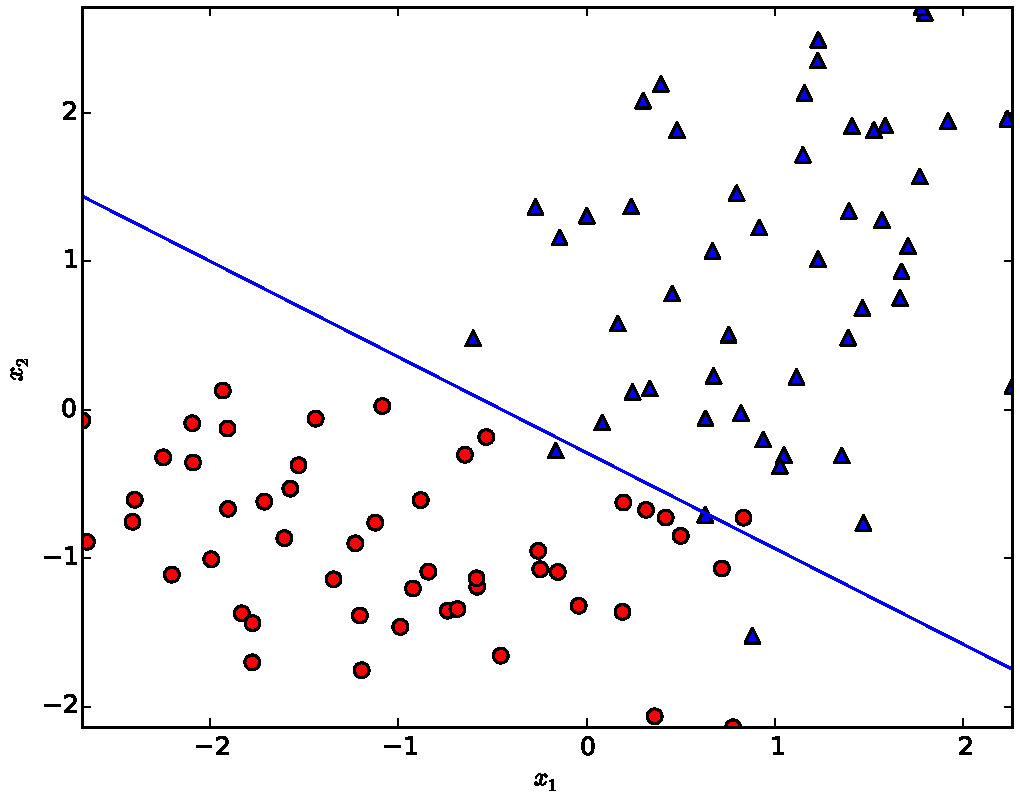
\includegraphics[width=7cm]{figures/perceptron-classification.pdf} % see code/perceptron.py
\end{center}

\end{frame}

% -----------------------------------------------------------------------------

\begin{frame}
\frametitle{Multilayer Perceptrons}
\framesubtitle{The Perceptron -- Limitations}

Only two classes\\\medskip % but there are extension to multiple classes
Linear decision boundaries\\\medskip % and these are not optimal in terms of margin, as opposed to SVM (but this applies to the MLP as well)
Learning never converges for non-separable data % so if we don't know whether our training data is linearly separable, we are in trouble

\end{frame}

% -----------------------------------------------------------------------------

\begin{frame}
\frametitle{Multilayer Perceptrons}
\framesubtitle{Two-Layer Architecture}

% here we only cover the standard two-layer architecture, which is the most common for "traditional MLPs" as they can encode any continuous decision boundary, as long as the number of hidden units is large enough. however, the architecture can be arbitrary as long as all nonlinearities are differentiable and there are no closed directed cycles in the graph

Replace $f$ with continuous nonlinearity (\eg $\tanh(\cdot)$)\\\medskip % differentiable
Introduce layer of $M$ such \enquote{Perceptrons} (hidden units)\\\medskip % no longer perceptrons but logistic regression models after replacing f, hence the quotes
Hidden units connected to layer of $K$ output units

\begin{center}
	\copyrightbox[b]
	{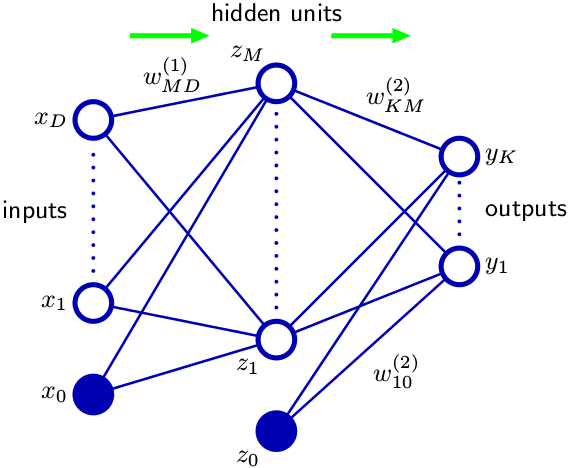
\includegraphics[width=4.5cm]{figures/two-layer-mlp.png}}
	{\centering Image from \cite{bishop2006}}
\end{center}

\end{frame}

% -----------------------------------------------------------------------------

\begin{frame}
\frametitle{Multilayer Perceptrons}
\framesubtitle{Two-Layer Architecture}

Output of $m$th hidden unit is $z_m(\vx)=f(\vw_m^\top\vx)$\\\medskip
Bias $b$ included in $\vw$ and $\vx$, $w_0=b$, $x_0=1$

\bigskip
\begin{center}
	\copyrightbox[b]
	{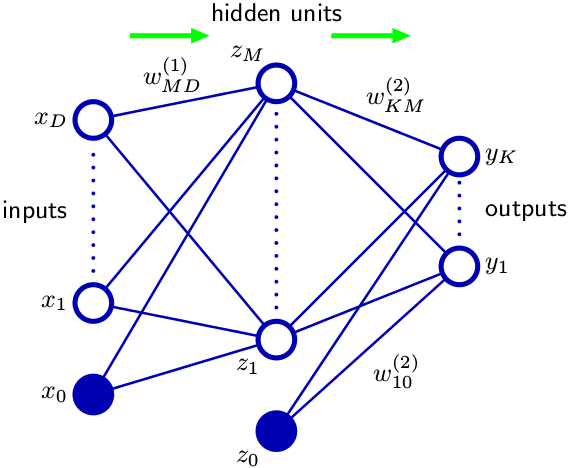
\includegraphics[width=4.5cm]{figures/two-layer-mlp.png}}
	{\centering Image from \cite{bishop2006}}
\end{center}

\end{frame}

% -----------------------------------------------------------------------------

\begin{frame}
\frametitle{Multilayer Perceptrons}
\framesubtitle{Two-Layer Architecture}

Output of $k$th output unit is $y_k(\vz)=g(\vw_k^\top\vz)$\\\medskip % this again includes the bias
Choice of $g$ depends on problem (regression, classification) % identity for regression, softmax for classification; must be differentiable

\bigskip
\begin{center}
	\copyrightbox[b]
	{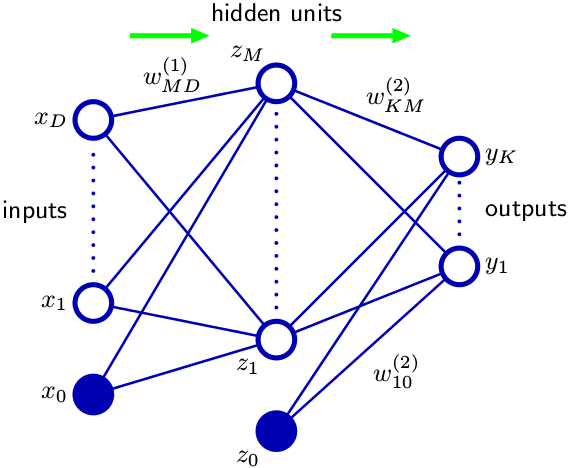
\includegraphics[width=4.5cm]{figures/two-layer-mlp.png}}
	{\centering Image from \cite{bishop2006}}
\end{center}

\end{frame}

% -----------------------------------------------------------------------------

\begin{frame}
\frametitle{Multilayer Perceptrons}
\framesubtitle{Two-Layer Architecture}

Both $f$ and $g$ are differentiable
\begin{itemize}
	\item Learn $\vw$ using gradient descent % here w contains all weights / the error function to minimize depends on the task; for regression we minimize the sum of squared residuals
	\item Gradients evaluated via error backpropagation % no details here, check bishop2006, for example
\end{itemize}

\end{frame}

% so we 

% -----------------------------------------------------------------------------

\begin{frame}
\frametitle{The Pylearn2 Library}

Machine learning library with focus on DL\\\medskip
Written in Python, but interaction mostly in YAML\\\medskip
Open-source: \url{https://github.com/lisa-lab/pylearn2}

\end{frame}

% -----------------------------------------------------------------------------

\begin{frame}
\frametitle{The Pylearn2 Library}
\framesubtitle{MLP Regression Example}

We will use pylearn2 to train a MLP for regression

\medskip
\begin{center}
	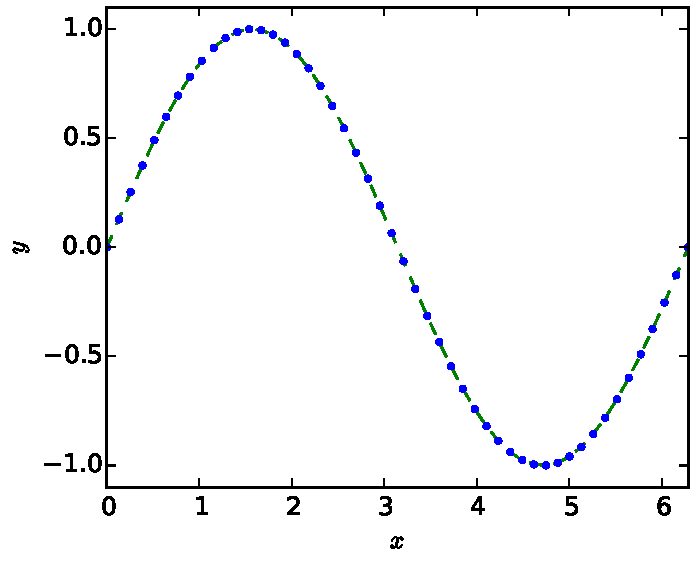
\includegraphics[width=6cm]{figures/mlp-input.pdf} % see code/mlp_gen_data_regression.py
\end{center}

\end{frame}

% -----------------------------------------------------------------------------

\begin{frame}[fragile]
\frametitle{The Pylearn2 Library}
\framesubtitle{MLP Regression Example}

% irange means "init weights randomly from [-irange,+irange]"
% linear layer means g() = identity

\begin{minted}[fontsize=\footnotesize]{yaml}
model: !obj:pylearn2.models.mlp.MLP {
    nvis: 1, # one input unit x
    layers: [ # two layers
        !obj:pylearn2.models.mlp.Tanh { # tanh activations for hidden units
            dim: 3, # use M=3 hidden units
            layer_name: 'hidden',
            irange: 1
        },
        !obj:pylearn2.models.mlp.Linear { # linear output layer for regression
            dim: 1, # one output unit, K=1 
            layer_name: 'out',
            irange: 1
        }
    ]
}
\end{minted}

\end{frame}

% -----------------------------------------------------------------------------

% see code/mlp_regression.yaml for the full code

\begin{frame}[fragile]
\frametitle{The Pylearn2 Library}
\framesubtitle{MLP Regression Example}

\begin{minted}[fontsize=\footnotesize]{yaml}
# dataset contains the (x,y) pairs from the previous figure
dataset: &train !pkl: 'mlp_data_regression.pkl',
# train using batch gradient descent
algorithm: !obj:pylearn2.training_algorithms.bgd.BGD {
    conjugate: 1,
    batch_size: 50,
    line_search_mode: 'exhaustive',
    termination_criterion: !obj:pylearn2.termination_criteria.EpochCounter {
        max_epochs: 100 # train for 100 epochs
    }
}
\end{minted}

\end{frame}

% -----------------------------------------------------------------------------

\begin{frame}
\frametitle{The Pylearn2 Library}
\framesubtitle{MLP Regression Example}

Full example: \url{https://github.com/cpra/cvsp-vo-slides}

\medskip
\begin{center}
	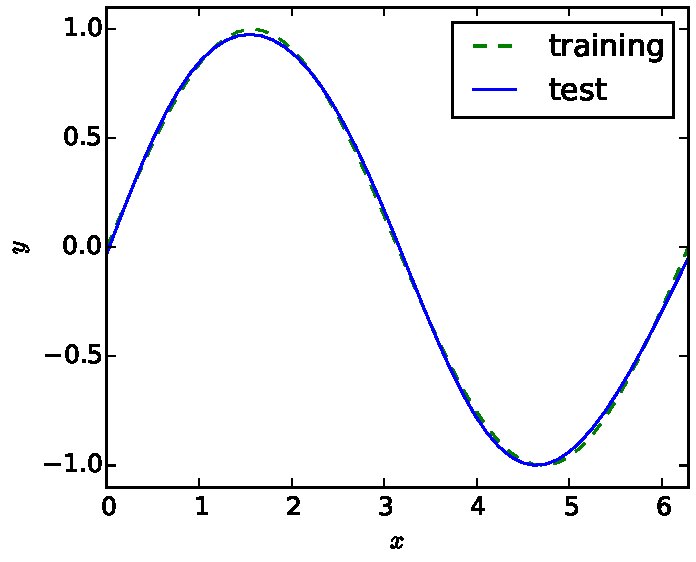
\includegraphics[width=6cm]{figures/mlp-regression.pdf} % see code/mlp_test_data_regression.py
\end{center}

\end{frame}

% -----------------------------------------------------------------------------

\begin{frame}[allowframebreaks=0.9]
\frametitle{Bibliography}

\printbibliography

\end{frame}

\end{document}